%%%%%%%%%%%%%%%%%%%%%%%%%%%%%%%%%%%%%%%%%%%%%%%%%%%%%%%
% A template for Wiley article submissions.
% Developed by Overleaf. 
%
% Please note that whilst this template provides a 
% preview of the typeset manuscript for submission, it 
% will not necessarily be the final publication layout.
%
% Usage notes:
% The "blind" option will make anonymous all author, affiliation, correspondence and funding information.
% Use "num-refs" option for numerical citation and references style.
% Use "alpha-refs" option for author-year citation and references style.

\documentclass[alpha-refs]{wiley-article-03v}
% \documentclass[blind,num-refs]{wiley-article}

% Add additional packages here if required
\usepackage{siunitx}

% For figures
\usepackage{graphics}

%For captions - even though template has complex caption commands
\usepackage[labelfont=bf,justification=centering]{caption}
\usepackage[font=small,labelfont=bf]{subcaption}
\captionsetup[sub]{font=tiny,labelfont={bf,sf}}

%% For figures numbered by section
\usepackage{chngcntr}
\counterwithin{figure}{section}
\counterwithin{table}{section}

%% Additional links for hyperref
\usepackage[unicode=true,pdfusetitle,
 bookmarks=false,bookmarksnumbered=false,bookmarksopen=true,bookmarksopenlevel=2,
 breaklinks=false,pdfborder={0 0 1},backref=false,colorlinks=false]
 {hyperref}
\hypersetup{pdfstartview={XYZ null null 1}}

\usepackage[backend=bibtex,
			natbib=true, 
			style=chicago-authordate]{biblatex}
\addbibresource{Returns.bib}

\usepackage{array}
\usepackage{longtable}
%\usepackage{fullpage}

\usepackage{lmodern}
\newcommand{\graph}[3]{
\raisebox{-#1mm}{\includegraphics[height=#2em,width=3cm]{#3}}
}

\usepackage{booktabs} % for vertically partitioned table


%%%%%%%%#################################################################################%%%%%%%%%%%%%%%%%%%%%%%%%%%%%

% Update article type if known
\papertype{WORLD BANK EDUCATION GLOBAL PRACTICE}
% Include section in journal if known, otherwise delete
\paperfield{Russian Federation: Analytical Services and Advisory Activity: 
P170978}

\title{Returns to Education in the Russian Federation: Variation across Regions }

% List acknowledgements here.
\fundinginfo{Thanks are due to the Higher School of Economics, Moscow for making the Russian Longitudinal Monitoring Study (RLMS) Household data readily available for reseachers around the world. The code used for this paper is made freely available for all researchers at \url{https://bitbucket.org/zagamog/edreru/src/master/}}

% Include full author names and degrees, when required by the journal.
% Use the \authfn to add symbols for additional footnotes and present addresses, if any. Usually start with 1 for notes about author contributions; then continuing with 2 etc if any author has a different present address.

\author[*]{Ekaterina Melianova}
\author[*]{\hspace{-1em}Suhas Parandekar}
\author[*]{\hspace{-1em}Harry Patrinos}
\author[*]{\hspace{-1em}Art\"{e}m Volgin}

% List abbreviations here, if any. Please note that it is preferred that abbreviations be defined at the first instance they appear in the text, rather than creating an abbreviations list.
\acks{\begin{normalsize}
\emph{Country Director:} Renaud Seligman; \emph{Regional Director:} Fadia Saadah; \emph{Practice Manager:} Harry Patrinos; \emph{Program Leader:} Dorota Nowak; \emph{Peer Reviewers}: Cristian Aedo; Ruslan Yemtsov; Husein Abdul-Hamid; \emph{Team members:} Polina Zavalina; Zhanna Terlyga. Thanks to seminar participants at the World Bank Moscow office on Jan. 29, 2020 for useful feedback. Any errors are a responsibility of the authors.
\end{normalsize}
\vspace{-0.2in}}

%\contrib[\authfn{1}]{Equally contributing authors.}

% Include full affiliation details for all authors
\affil[*]{Education Global Practice, Europe and Central Asia}

%\corraddress{Author One PhD, Department, Institution, City, State or Province, Postal Code, Country}
\corremail{sparandekar@worldbank.org}

%\presentadd[\authfn{2}]{Department, Institution, City, State or Province, Postal Code, Country}

% Include the name of the author that should appear in the running header
\runningauthor{P170978: WP03 - Variation across Regions}

\begin{document}

\maketitle

\begin{abstract}
This is a generic template designed for use by multiple journals, which includes several options for customization. Please consult the author guidelines for the journal to which you are submitting in order to confirm that your manuscript will comply with the journal's requirements. Please replace this text with your abstract.

% Please include a maximum of seven keywords
\keywords{keyword 1, \emph{keyword 2}, keyword 3, keyword 4, keyword 5, keyword 6, keyword 7}
\end{abstract}


\section{Regional Returns to Education in the Russian Federation: Role of access to Vocational and Higher Education}

\subsection{Data}
To estimate returns to education in Russian regions, we use the most recent (2018) round of the Statistical Survey of Income and Participation in Social Programs, collected by Rosstat. The primary purpose of the Rosstat survey was to obtain statistical information, reflecting the role of wages, income from self-employment, property income, pensions, and social benefits in ensuring the material well-being of families. The survey contains data on trends in income and poverty variation among households with different socio-economic status. There are also variables on people's participation in social programs, their pension and health insurance, material and social security of low-income families, and the impact of social policy measures on people's well-being. The sample selected for the empirical modeling is identical to the one used for the RLMS analysis: individuals aged 25-64 who are out of school and have positive labor market experience and income.

\subsection{Methods}

The classical Mincerian equation (described in the previous sections) is the main focus in the regional investigation of returns to education in Russia: in this section we look at how these returns vary across regions. Additionally, we explore the determinants of the established variation through a random effects regression analysis.  The equations of interest are as follows:

\textbf{First level:}
\begin{flalign}\label{eq:4.1} 
Log(Wage)_{ij} = b_{0j} + b_{1j}\cdot Educ + b_{2j}\cdot Exp + b_{3j}\cdot Exp^2 + b_{4j}\cdot Gender + \epsilon_{ij} &&
\end{flalign}

\textbf{Second Level:}
\begin{flalign}\label{eq:4.2} 
b_{0j} = \gamma_{00} + \gamma_{0n}\cdot Z + u_{00} ;&&
b_{1j} = \gamma_{10} + \gamma_{1n}\cdot Z + u_{10} ;&&
b_{ij} = \gamma_{i0} \quad for \quad i \neq 0   &&
\end{flalign}
 
\noindent
where an individual $i$ is nested withing a region $j$, $Log(Wage)$ is a logarithm of monthly wage, $Educ$ stands for highest attained level of education, $Exp$ and $Exp^2$ reflect the years of working experience and its quadratic term respectively, $Gender$ is a dummy variable for gender, $Z$ is an $n\times i$ matrix of regional characteristics, $\epsilon$ and $u_{00}$, $u_{10}$ are the first- and second-level errors respectively.

The random effects models were estimated using restricted maximum likelihood (REML). Individual Wald tests and likelihood ratio tests were exploited to evaluate the significance of fixed and random effects, respectively. Weights were used in the modeling to ensure the representativeness of the sample across Russian regions (the weighting variable was divided by 1000 to allow the convergence of the multilevel models). 

\subsubsection{Left Hand Side (LHS) variable}
Similar to the previous analyses, the outcome to be investigated is the logarithm of monthly monetary remuneration before income tax payment at the main place of work.

\subsubsection{Right Hand Side (RHS) variables}
Education, experience, and gender are the first-level  variables. Education is included in the random effects models as the focus of interest with a set of regional level variables - equation \ref{eq:4.2}. 

The random effects model seeks to estimate the magnitude of influence of regional level educational quantity and educational quality measures to explain the variation in returns to education across Russian regions. To measure educational quanity or access, we use the number of students enrolled in vocational education per 10,000 residents and the number of students enrolled in higher education per 10,000 residents. As a measure of educational quality, we use standard deviations from the national mean of the Russian school-leaving and university entrance examination, the EGE. We also add control variables regarding economic development and the labor market - these are respectively the gross regional product, the level of urbanization, the regional unemployment level and the the share of employment in jobs related to natural resource exploitation. Table \ref{tab:4.1} demonstrates the descriptive statistics by region.

\hspace{-1in}
\fontsize{9}{11}{
	\selectfont
	\setlength{\tabcolsep}{2pt}
	\begin{longtable}{lcccccccccc}
		\caption{Descriptive Statistics for Regions in Russia, Rosstat 2018}
		\label{tab:4.1}\\
&  & \multicolumn{2}{c}{\textbf{Wage}} & \multicolumn{2}{c}{\textbf{Experience}} & \multicolumn{3}{c}{\textbf{Education}, \%} & \multicolumn{2}{c}{\textbf{Gender}, \%} \\ 
	    \hline
Regions & N & mean & sd & mean & sd & SE & VE & HE & Males & Females  \\
		\hline
		\endhead
		Altayskiy Kray  & $\phantom{0}4646$ & $22127.6$ & $11952.2$ & $\phantom{000}23.6$ & $\phantom{000}11.0$ & $17.456$ & $54.50$ & $28.05$ & $48.90$ & $51.10$ \\
		Amurskaya Oblast  & $\phantom{0}2557$ & $33441.2$ & $17409.0$ & $\phantom{000}23.2$ & $\phantom{000}11.2$ & $16.347$ & $50.65$ & $33.01$ & $49.59$ & $50.41$ \\
		Arkhangelskaya Oblast  & $\phantom{0}3183$ & $33438.1$ & $16884.2$ & $\phantom{000}22.6$ & $\phantom{000}10.6$ & $12.692$ & $54.95$ & $32.36$ & $44.17$ & $55.83$ \\
		Astrakhanskaya Oblast  & $\phantom{0}2836$ & $26474.1$ & $13737.6$ & $\phantom{000}23.0$ & $\phantom{000}11.3$ & $13.646$ & $55.08$ & $31.28$ & $50.99$ & $49.01$ \\
		Belgorodskaya Oblast  & $\phantom{0}3692$ & $26281.0$ & $10811.9$ & $\phantom{000}23.8$ & $\phantom{000}11.1$ & $12.351$ & $54.47$ & $33.18$ & $49.76$ & $50.24$ \\
		Bryanskaya Oblast  & $\phantom{0}3087$ & $22482.3$ & $\phantom{0}9634.1$ & $\phantom{000}23.5$ & $\phantom{000}10.9$ & $19.631$ & $50.66$ & $29.71$ & $48.66$ & $51.34$ \\
		Chechenskaya Respublika  & $\phantom{0}2010$ & $27718.4$ & $11793.2$ & $\phantom{000}18.7$ & $\phantom{000}10.6$ & $25.721$ & $26.37$ & $47.91$ & $65.37$ & $34.63$ \\
		Chelyabinskaya Oblast  & $\phantom{0}6717$ & $27990.8$ & $14280.9$ & $\phantom{000}23.9$ & $\phantom{000}11.2$ & $12.104$ & $54.53$ & $33.36$ & $47.39$ & $52.61$ \\
		Chukotskiy Aok  & $\phantom{0}1535$ & $65574.1$ & $32370.8$ & $\phantom{000}23.6$ & $\phantom{000}10.6$ & $13.941$ & $46.06$ & $40.00$ & $43.97$ & $56.03$ \\
		Chuvashskaya Respublika  & $\phantom{0}3248$ & $21453.7$ & $12602.2$ & $\phantom{000}24.3$ & $\phantom{000}11.0$ & $19.119$ & $50.80$ & $30.08$ & $50.18$ & $49.82$ \\
		Evreyskaya AOb  & $\phantom{0}1536$ & $28532.1$ & $17385.1$ & $\phantom{000}23.8$ & $\phantom{000}11.2$ & $22.005$ & $50.33$ & $27.67$ & $50.00$ & $50.00$ \\
		Irkutskaya Oblast  & $\phantom{0}4686$ & $29967.6$ & $17443.1$ & $\phantom{000}22.3$ & $\phantom{000}11.2$ & $17.520$ & $47.06$ & $35.42$ & $47.57$ & $52.43$ \\
		Ivanovskaya Oblast  & $\phantom{0}2876$ & $24881.8$ & $12496.8$ & $\phantom{000}23.3$ & $\phantom{000}10.9$ & $20.341$ & $49.90$ & $29.76$ & $47.77$ & $52.23$ \\
		Kabardino-Balkarskaya Res.  & $\phantom{0}2006$ & $23592.3$ & $10766.2$ & $\phantom{000}21.7$ & $\phantom{000}11.6$ & $21.137$ & $40.53$ & $38.33$ & $52.04$ & $47.96$ \\
		Kaliningradskaya Oblast  & $\phantom{0}2838$ & $29749.2$ & $15489.1$ & $\phantom{000}23.5$ & $\phantom{000}11.4$ & $13.495$ & $52.40$ & $34.11$ & $50.07$ & $49.93$ \\
		Kaluzhskaya Oblast  & $\phantom{0}3155$ & $29662.1$ & $12879.5$ & $\phantom{000}24.1$ & $\phantom{000}11.2$ & $13.312$ & $52.11$ & $34.58$ & $47.92$ & $52.08$ \\
		Kamchatskaya Kray  & $\phantom{0}2203$ & $51160.5$ & $29997.7$ & $\phantom{000}23.1$ & $\phantom{000}11.2$ & $13.118$ & $42.99$ & $43.89$ & $47.89$ & $52.11$ \\
		Karachayevo-Cherkessiya  & $\phantom{0}1510$ & $22900.6$ & $12540.8$ & $\phantom{000}22.0$ & $\phantom{000}11.8$ & $17.152$ & $40.07$ & $42.78$ & $48.01$ & $51.99$ \\
		Kemerovskaya Oblast  & $\phantom{0}5056$ & $26287.0$ & $13774.4$ & $\phantom{000}23.6$ & $\phantom{000}11.3$ & $18.137$ & $52.99$ & $28.88$ & $48.04$ & $51.96$ \\
		Khabarovskiy Kray  & $\phantom{0}3731$ & $42008.8$ & $21837.8$ & $\phantom{000}22.3$ & $\phantom{000}11.2$ & $11.900$ & $44.33$ & $43.77$ & $46.15$ & $53.85$ \\
		Khanty-Mansiyskiy Aok  & $\phantom{0}4335$ & $50837.9$ & $22261.7$ & $\phantom{000}22.8$ & $\phantom{000}10.5$ & $13.564$ & $46.78$ & $39.65$ & $49.60$ & $50.40$ \\
		Kirovskaya Oblast  & $\phantom{0}3284$ & $22941.0$ & $13674.6$ & $\phantom{000}25.1$ & $\phantom{000}11.2$ & $20.128$ & $55.33$ & $24.54$ & $47.69$ & $52.31$ \\
		Kostromskaya Oblast  & $\phantom{0}2518$ & $23993.1$ & $12090.9$ & $\phantom{000}23.6$ & $\phantom{000}11.1$ & $12.669$ & $61.28$ & $26.05$ & $47.82$ & $52.18$ \\
		Krasnodarskiy Kray  & $\phantom{0}8730$ & $32563.7$ & $17499.8$ & $\phantom{000}23.0$ & $\phantom{000}10.9$ & $15.888$ & $48.57$ & $35.54$ & $50.02$ & $49.98$ \\
		Krasnoyarskiy Kray  & $\phantom{0}5540$ & $33954.6$ & $21199.2$ & $\phantom{000}23.0$ & $\phantom{000}11.0$ & $21.588$ & $48.05$ & $30.36$ & $49.64$ & $50.36$ \\
		Kurganskaya Oblast  & $\phantom{0}2468$ & $20896.9$ & $11539.5$ & $\phantom{000}24.4$ & $\phantom{000}10.7$ & $21.394$ & $52.47$ & $26.13$ & $48.38$ & $51.62$ \\
		Kurskaya Oblast  & $\phantom{0}2956$ & $23622.6$ & $11475.0$ & $\phantom{000}23.9$ & $\phantom{000}11.0$ & $14.783$ & $52.17$ & $33.05$ & $50.30$ & $49.70$ \\
		Leningradskaya Oblast  & $\phantom{0}4506$ & $32124.3$ & $17227.4$ & $\phantom{000}24.2$ & $\phantom{000}11.5$ & $\phantom{0}7.723$ & $54.77$ & $37.51$ & $46.03$ & $53.97$ \\
		Lipetskaya Oblast  & $\phantom{0}2869$ & $25037.8$ & $10813.5$ & $\phantom{000}24.1$ & $\phantom{000}11.0$ & $13.106$ & $53.82$ & $33.08$ & $49.60$ & $50.40$ \\
		Magadanskaya Oblast  & $\phantom{0}1841$ & $51000.8$ & $23729.4$ & $\phantom{000}24.1$ & $\phantom{000}11.4$ & $18.523$ & $43.02$ & $38.46$ & $43.24$ & $56.76$ \\
		Moscow  & $29921$ & $66263.5$ & $26437.9$ & $\phantom{000}20.8$ & $\phantom{000}10.8$ & $\phantom{0}4.953$ & $32.18$ & $62.86$ & $47.06$ & $52.94$ \\
		Moskovskaya Oblast  & $13431$ & $46725.1$ & $20563.7$ & $\phantom{000}22.6$ & $\phantom{000}11.4$ & $10.975$ & $39.13$ & $49.89$ & $47.51$ & $52.49$ \\
		Murmanskaya Oblast  & $\phantom{0}3078$ & $43992.5$ & $28841.9$ & $\phantom{000}23.4$ & $\phantom{000}11.2$ & $12.801$ & $50.45$ & $36.74$ & $49.84$ & $50.16$ \\
		Nenetskiy Aok  & $\phantom{0}1118$ & $54467.3$ & $23147.1$ & $\phantom{000}22.6$ & $\phantom{000}10.8$ & $17.263$ & $49.73$ & $33.01$ & $39.98$ & $60.02$ \\
		Nizhegorodskaya Oblast  & $\phantom{0}6139$ & $30912.9$ & $13291.8$ & $\phantom{000}23.4$ & $\phantom{000}11.2$ & $16.941$ & $49.31$ & $33.75$ & $47.42$ & $52.58$ \\
		Novgorodskaya Oblast  & $\phantom{0}2673$ & $26856.0$ & $12683.0$ & $\phantom{000}24.6$ & $\phantom{000}11.2$ & $15.638$ & $55.74$ & $28.62$ & $45.16$ & $54.84$ \\
		Novosibirskaya Oblast  & $\phantom{0}5374$ & $29229.9$ & $14687.7$ & $\phantom{000}23.9$ & $\phantom{000}11.6$ & $16.561$ & $49.33$ & $34.11$ & $47.06$ & $52.94$ \\
		Omskaya Oblast  & $\phantom{0}3978$ & $25337.5$ & $14613.1$ & $\phantom{000}23.6$ & $\phantom{000}10.9$ & $22.197$ & $51.31$ & $26.50$ & $51.11$ & $48.89$ \\
		Orenburgskaya Oblast  & $\phantom{0}4190$ & $24207.0$ & $12519.9$ & $\phantom{000}23.3$ & $\phantom{000}11.0$ & $15.131$ & $53.68$ & $31.19$ & $51.29$ & $48.71$ \\
		Orlovskaya Oblast  & $\phantom{0}2424$ & $21901.2$ & $10561.0$ & $\phantom{000}24.7$ & $\phantom{000}11.1$ & $15.017$ & $50.66$ & $34.32$ & $46.99$ & $53.01$ \\
		Penzenskaya Oblast  & $\phantom{0}3103$ & $23478.4$ & $10982.9$ & $\phantom{000}24.2$ & $\phantom{000}11.0$ & $20.722$ & $51.40$ & $27.88$ & $51.02$ & $48.98$ \\
		Permskiy Krai  & $\phantom{0}5290$ & $29176.6$ & $14449.4$ & $\phantom{000}23.4$ & $\phantom{000}11.0$ & $13.894$ & $58.32$ & $27.79$ & $48.17$ & $51.83$ \\
		Primorskiy Kray  & $\phantom{0}4104$ & $37839.9$ & $18420.2$ & $\phantom{000}23.8$ & $\phantom{000}11.3$ & $14.985$ & $52.97$ & $32.04$ & $49.98$ & $50.02$ \\
		Pskovskaya Oblast  & $\phantom{0}2382$ & $23838.4$ & $12015.3$ & $\phantom{000}25.0$ & $\phantom{000}11.0$ & $17.632$ & $55.33$ & $27.04$ & $48.11$ & $51.89$ \\
		Respublika Adygeya  & $\phantom{0}2013$ & $21350.3$ & $10505.9$ & $\phantom{000}23.4$ & $\phantom{000}11.3$ & $20.666$ & $43.67$ & $35.67$ & $49.53$ & $50.47$ \\
		Respublika Altay  & $\phantom{0}1381$ & $20285.3$ & $12029.5$ & $\phantom{000}23.0$ & $\phantom{000}10.6$ & $23.027$ & $45.26$ & $31.72$ & $43.08$ & $56.92$ \\
		Respublika Bashkortostan  & $\phantom{0}7126$ & $31100.8$ & $15175.2$ & $\phantom{000}23.4$ & $\phantom{000}11.0$ & $12.167$ & $56.67$ & $31.17$ & $51.98$ & $48.02$ \\
		Respublika Buryatia  & $\phantom{0}2469$ & $29536.3$ & $17237.4$ & $\phantom{000}22.1$ & $\phantom{000}10.6$ & $17.173$ & $45.61$ & $37.22$ & $48.12$ & $51.88$ \\
		Respublika Crimea  & $\phantom{0}2895$ & $19916.2$ & $\phantom{0}9743.9$ & $\phantom{000}22.8$ & $\phantom{000}11.0$ & $21.244$ & $43.90$ & $34.85$ & $52.99$ & $47.01$ \\
		Respublika Dagestan  & $\phantom{0}3388$ & $26377.3$ & $11971.9$ & $\phantom{000}23.0$ & $\phantom{000}10.7$ & $30.519$ & $30.79$ & $38.70$ & $55.99$ & $44.01$ \\
		Respublika Ingushetiya  & $\phantom{0}1207$ & $23740.2$ & $10168.5$ & $\phantom{000}18.2$ & $\phantom{0000}9.6$ & $10.025$ & $18.89$ & $71.09$ & $61.14$ & $38.86$ \\
		Respublika Kalmykiya  & $\phantom{0}1751$ & $18568.8$ & $11749.1$ & $\phantom{000}23.6$ & $\phantom{000}11.4$ & $15.762$ & $40.89$ & $43.35$ & $46.43$ & $53.57$ \\
		Respublika Karelia  & $\phantom{0}2164$ & $28510.2$ & $16639.5$ & $\phantom{000}23.7$ & $\phantom{000}10.8$ & $17.144$ & $55.45$ & $27.40$ & $47.00$ & $53.00$ \\
		Respublika Khakasiya  & $\phantom{0}2064$ & $27288.1$ & $16613.3$ & $\phantom{000}23.3$ & $\phantom{000}11.1$ & $22.045$ & $51.11$ & $26.84$ & $50.97$ & $49.03$ \\
		Respublika Komi  & $\phantom{0}2972$ & $35891.6$ & $21554.4$ & $\phantom{000}23.8$ & $\phantom{000}11.0$ & $16.689$ & $53.47$ & $29.85$ & $46.67$ & $53.33$ \\
		Respublika Mariy El  & $\phantom{0}2486$ & $21133.1$ & $11941.6$ & $\phantom{000}24.1$ & $\phantom{000}11.2$ & $18.785$ & $52.98$ & $28.24$ & $47.87$ & $52.13$ \\
		Respublika Mordovia  & $\phantom{0}2236$ & $21221.0$ & $10837.3$ & $\phantom{000}23.1$ & $\phantom{000}11.2$ & $15.519$ & $49.11$ & $35.38$ & $48.35$ & $51.65$ \\
		Respublika Saha (Yakutia)  & $\phantom{0}3243$ & $45763.1$ & $25001.6$ & $\phantom{000}23.2$ & $\phantom{000}11.3$ & $18.440$ & $45.76$ & $35.80$ & $46.69$ & $53.31$ \\
		Respublika Severnaya Osetiya  & $\phantom{0}2114$ & $22993.1$ & $12762.5$ & $\phantom{000}21.8$ & $\phantom{000}11.3$ & $12.677$ & $40.92$ & $46.40$ & $48.91$ & $51.09$ \\
		Respublika Tatarstan  & $\phantom{0}7212$ & $30327.9$ & $12928.8$ & $\phantom{000}23.5$ & $\phantom{000}11.1$ & $18.691$ & $48.64$ & $32.67$ & $51.48$ & $48.52$ \\
		Respublika Tyva  & $\phantom{0}1704$ & $23421.9$ & $16851.3$ & $\phantom{000}21.4$ & $\phantom{000}10.0$ & $19.777$ & $44.78$ & $35.45$ & $40.43$ & $59.57$ \\
		Rostovskaya Oblast  & $\phantom{0}6985$ & $28287.2$ & $12779.9$ & $\phantom{000}23.1$ & $\phantom{000}11.0$ & $15.476$ & $48.03$ & $36.49$ & $50.68$ & $49.32$ \\
		Ryazanskaya Oblast  & $\phantom{0}2609$ & $25889.2$ & $11760.9$ & $\phantom{000}24.7$ & $\phantom{000}11.1$ & $12.457$ & $59.37$ & $28.17$ & $49.18$ & $50.82$ \\
		Saint-Petersburg  & $11352$ & $48520.8$ & $23771.0$ & $\phantom{000}22.8$ & $\phantom{000}11.4$ & $\phantom{0}5.259$ & $38.15$ & $56.59$ & $46.04$ & $53.96$ \\
		Sakhalinskaya Oblast  & $\phantom{0}2258$ & $50325.1$ & $25563.0$ & $\phantom{000}23.6$ & $\phantom{000}11.2$ & $17.493$ & $48.23$ & $34.28$ & $46.94$ & $53.06$ \\
		Samarskaya Oblast  & $\phantom{0}6275$ & $32584.4$ & $15015.6$ & $\phantom{000}23.8$ & $\phantom{000}11.1$ & $11.331$ & $47.87$ & $40.80$ & $47.71$ & $52.29$ \\
		Saratovskaya Oblast  & $\phantom{0}4572$ & $23698.6$ & $12322.4$ & $\phantom{000}23.7$ & $\phantom{000}10.8$ & $14.961$ & $50.22$ & $34.82$ & $50.42$ & $49.58$ \\
		Sevastopol  & $\phantom{0}1489$ & $24811.3$ & $13498.9$ & $\phantom{000}22.4$ & $\phantom{000}11.2$ & $\phantom{0}9.671$ & $44.93$ & $45.40$ & $53.32$ & $46.68$ \\
		Smolenskaya Oblast  & $\phantom{0}2726$ & $25517.8$ & $12104.9$ & $\phantom{000}24.6$ & $\phantom{000}11.3$ & $14.380$ & $52.31$ & $33.31$ & $46.04$ & $53.96$ \\
		Stavropolskiy Kray  & $\phantom{0}4945$ & $25263.6$ & $12696.7$ & $\phantom{000}22.6$ & $\phantom{000}11.3$ & $16.946$ & $43.80$ & $39.25$ & $47.48$ & $52.52$ \\
		Sverdlovskaya Oblast  & $\phantom{0}7712$ & $35983.2$ & $15242.7$ & $\phantom{000}23.6$ & $\phantom{000}11.3$ & $16.779$ & $54.94$ & $28.28$ & $48.59$ & $51.41$ \\
		Tambovskaya Oblast  & $\phantom{0}2781$ & $22698.6$ & $10440.1$ & $\phantom{000}24.1$ & $\phantom{000}11.0$ & $16.397$ & $53.54$ & $30.06$ & $50.67$ & $49.33$ \\
		Tomskaya Oblast  & $\phantom{0}3074$ & $29580.6$ & $16745.7$ & $\phantom{000}22.1$ & $\phantom{000}11.1$ & $13.500$ & $47.56$ & $38.94$ & $46.78$ & $53.22$ \\
		Tulskaya Oblast  & $\phantom{0}3516$ & $27687.4$ & $11814.7$ & $\phantom{000}24.3$ & $\phantom{000}11.3$ & $17.491$ & $54.69$ & $27.82$ & $48.98$ & $51.02$ \\
		Tverskaya Oblast  & $\phantom{0}3157$ & $26310.0$ & $15025.1$ & $\phantom{000}25.5$ & $\phantom{000}11.1$ & $14.824$ & $56.57$ & $28.60$ & $44.73$ & $55.27$ \\
		Tyumenskaya Oblast  & $\phantom{0}3095$ & $31441.2$ & $17278.6$ & $\phantom{000}22.7$ & $\phantom{000}11.2$ & $16.123$ & $52.89$ & $30.99$ & $50.05$ & $49.95$ \\
		Udmurtskaya Respublika  & $\phantom{0}4073$ & $24044.6$ & $11540.9$ & $\phantom{000}23.9$ & $\phantom{000}11.3$ & $20.108$ & $51.04$ & $28.85$ & $46.99$ & $53.01$ \\
		Ul'yanovskaya Oblast  & $\phantom{0}3109$ & $23215.3$ & $10596.4$ & $\phantom{000}24.8$ & $\phantom{000}10.9$ & $19.170$ & $53.84$ & $26.99$ & $50.37$ & $49.63$ \\
		Vladimirskaya Oblast  & $\phantom{0}3502$ & $25001.4$ & $12605.8$ & $\phantom{000}24.5$ & $\phantom{000}11.4$ & $19.503$ & $50.77$ & $29.73$ & $46.49$ & $53.51$ \\
		Volgogradskaya Oblast  & $\phantom{0}4836$ & $24459.0$ & $12915.8$ & $\phantom{000}23.2$ & $\phantom{000}11.0$ & $15.881$ & $50.91$ & $33.21$ & $49.69$ & $50.31$ \\
		Vologodskaya Oblast  & $\phantom{0}2965$ & $28248.9$ & $16693.8$ & $\phantom{000}23.9$ & $\phantom{000}11.2$ & $17.302$ & $57.47$ & $25.23$ & $49.61$ & $50.39$ \\
		Voronezhskaya Oblast  & $\phantom{0}4348$ & $26261.9$ & $11813.9$ & $\phantom{000}23.6$ & $\phantom{000}11.5$ & $22.700$ & $43.38$ & $33.92$ & $48.37$ & $51.63$ \\
		Yamalo-Nenetskiy Aok  & $\phantom{0}3164$ & $69356.7$ & $28075.6$ & $\phantom{000}21.0$ & $\phantom{000}10.4$ & $10.683$ & $40.27$ & $49.05$ & $48.74$ & $51.26$ \\
		Yaroslavskaya Oblast  & $\phantom{0}3361$ & $30261.4$ & $14682.8$ & $\phantom{000}24.1$ & $\phantom{000}11.4$ & $16.215$ & $53.73$ & $30.05$ & $47.01$ & $52.99$ \\
		Zabaykalskiy Kray  & $\phantom{0}3017$ & $28336.6$ & $16350.4$ & $\phantom{000}23.0$ & $\phantom{000}10.6$ & $24.561$ & $47.40$ & $28.04$ & $47.07$ & $52.93$ \\
		\hline 
	\end{longtable}
}

\subsection{Estimation Results of Regional Analysis}
First, simple linear regression models were fitted to the observations in each region, and 95\% confidence intervals for the education variable coefficients were returned to examine the overall pattern of regional diversity in education payoffs. A visual inspection of Figure \ref{fig:4.1} is illustrative of the fact that Russian regions are rather heterogeneous in terms of premiums to education. Following the basic Mincerian equation, we present the results of the multilevel regression.

\begin{figure}[htp]
	\begin{minipage}[b]{.5\linewidth}
		\centering
		\hspace*{-0.4in}
		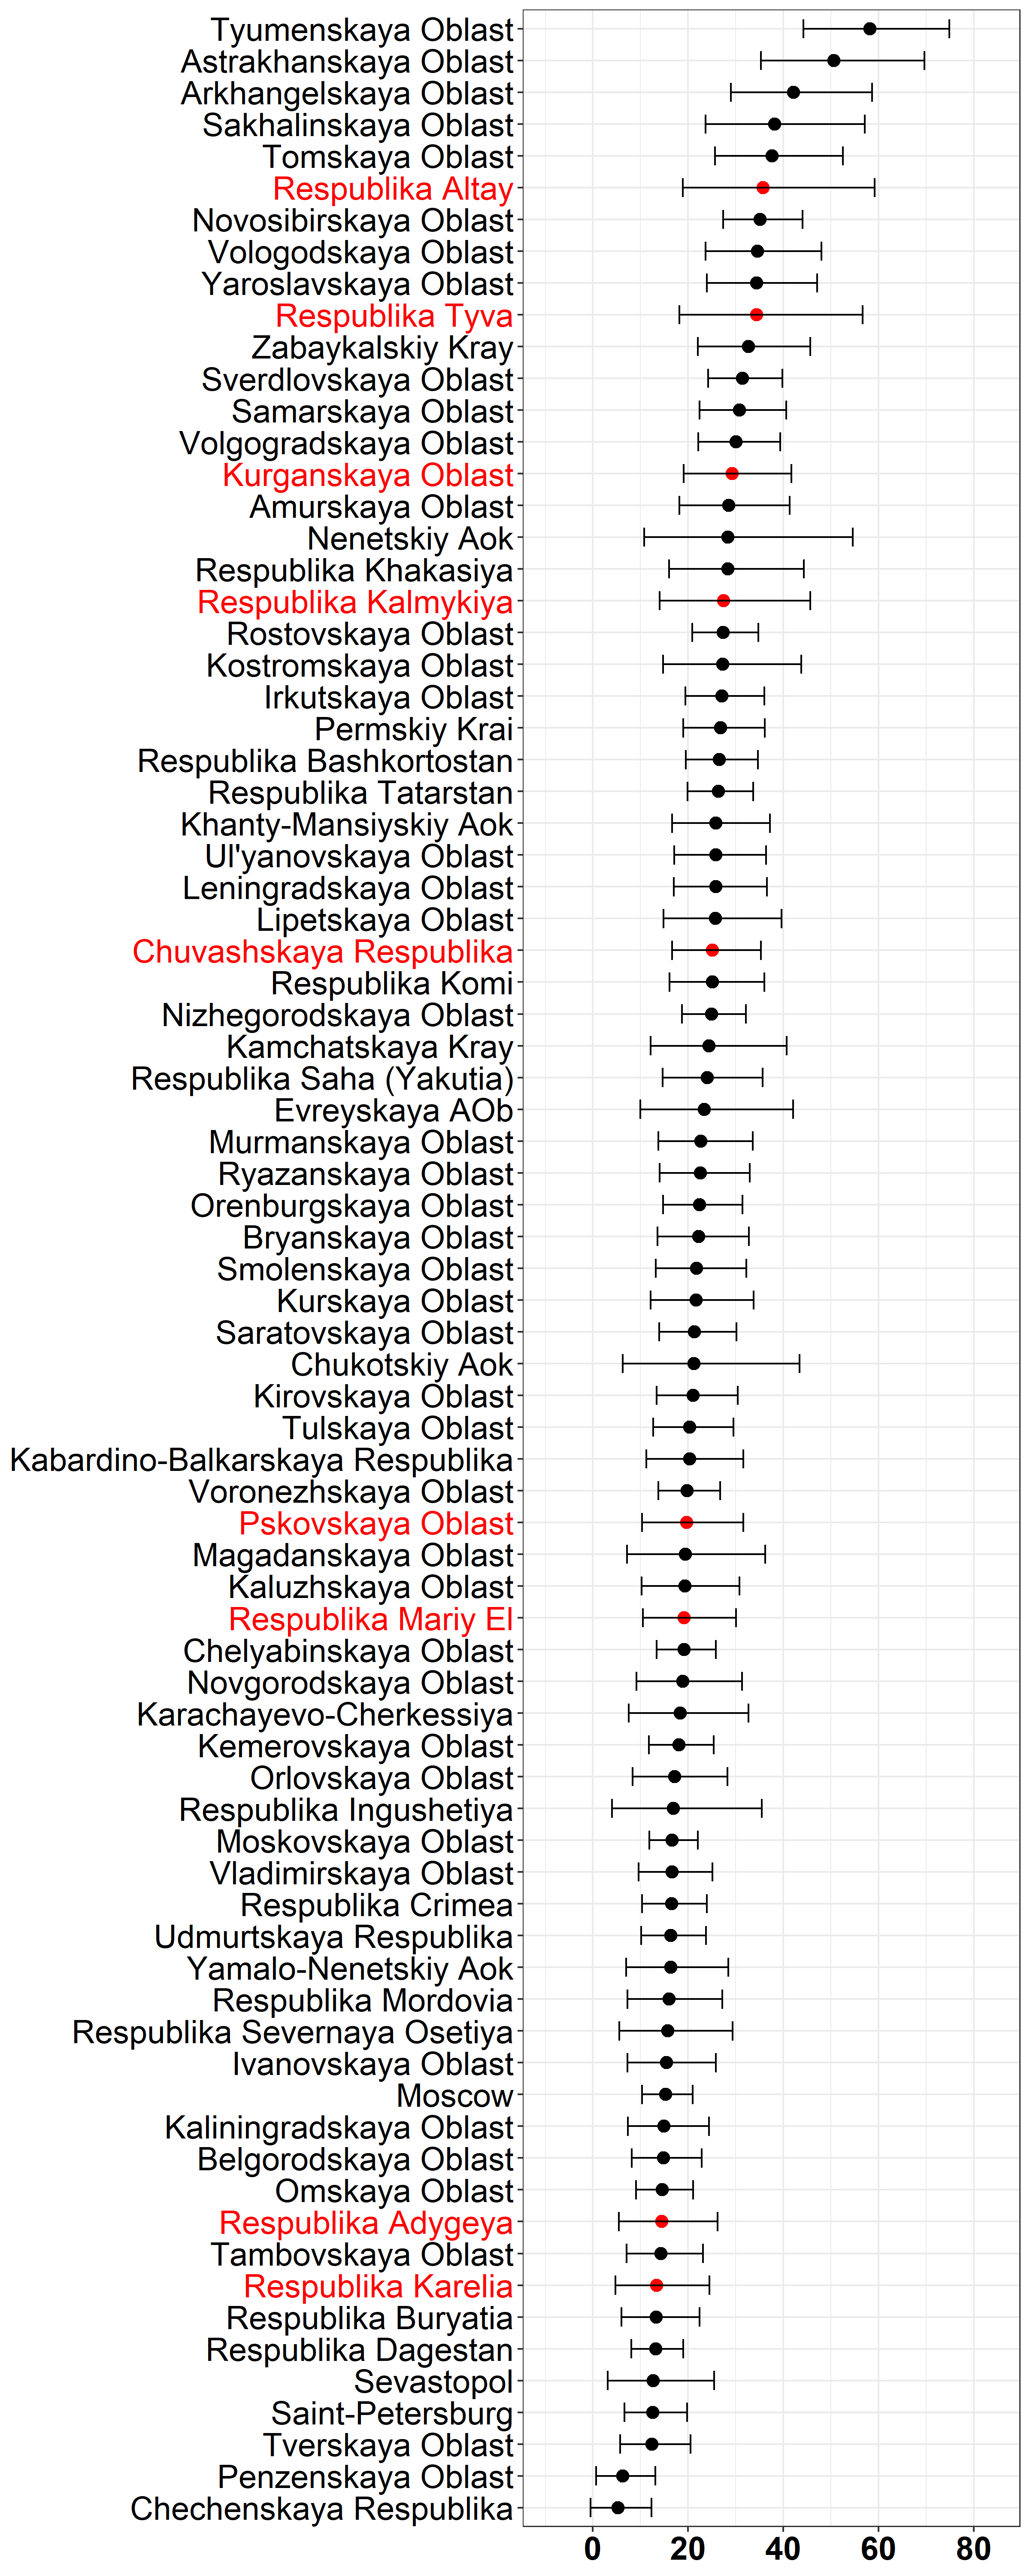
\includegraphics[width=250pt]{reg_he_18.png}
		% plot 1
		\subcaption{Higher Education}\label{}
	\end{minipage}
	\hfill
	\begin{minipage}[b]{.5\linewidth}
		\centering
		\hspace*{-0.2in}
		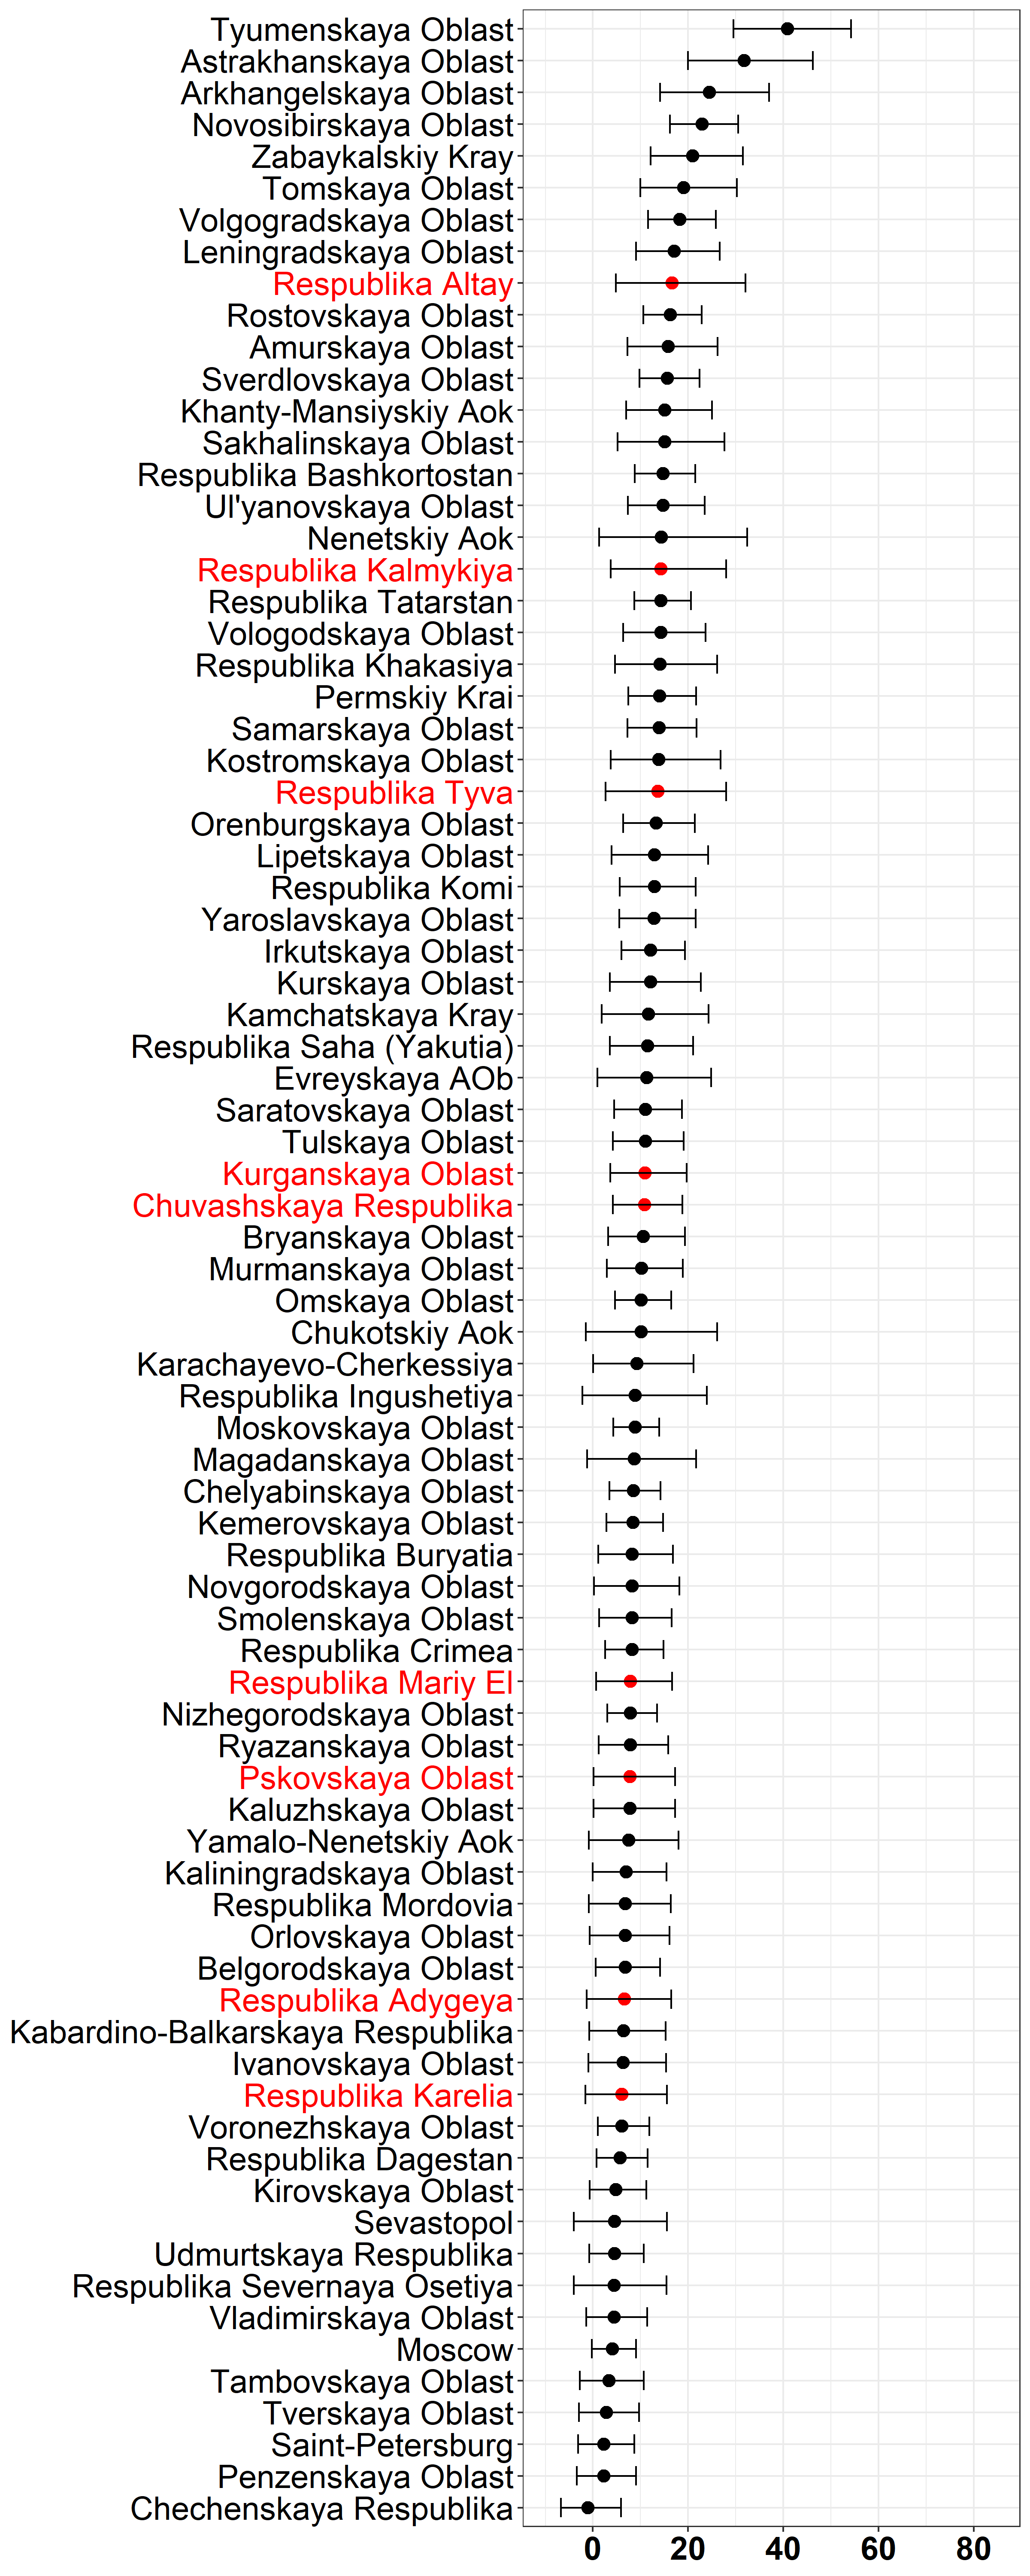
\includegraphics[width=250pt]{reg_ve_18.png}
		% plot 2
		\subcaption{Vocational Education}\label{}
	\end{minipage}
	\caption{Rates of Returns (Percentages) to Higher and Vocational Education in Russian Regions, Rosstat 2018}\label{fig:4.1}
\end{figure}

A two-level model without covariates was initially specified and indicated that the Intra-class Correlation (ICC) was equal to 16\%, i.e., 16\% of the variation in wage outcome was between regions. This is a high enough level to justify the estimation of a random effects model with covariates. Nested models comparison showed that there is a statistically significant regional variation in the effect of education on people's earnings ($-2\bigtriangleup LL(1) = 413.54, p < .001$).

Next, we examined the possible causes of this variation by adding the second-level independent variables and their interactions with education. The investigation revealed that none of the second-level characteristics are capable of changing the association between education and the amount of money Russians earn, except for \textit{the coverage by vocational education}. Substantively, it means that growth in the number of students covered by vocational programs leads to higher schooling premiums concerning both vocational and university education. As for the estimates obtained, sufficiently high vocational education coverage degree (when its standardized version is 1) corresponds to the average return rate of 30.6\%; medium vocational education coverage degree (when its standardized version is 0) corresponds to the average return rate of 35.8\%; low vocational education coverage degree (when its standardized version is -1) corresponds to the average return rate of 25.5\%. The interpretation of such a finding can imply that this quantity-related dimension of vocational education has the potential to serve as an instrument of boosting financial payoffs from post-secondary education in Russian regions. 


\printbibliography

\newpage
\section*{Appendix}
\addcontentsline{toc}{section}{Appendix}%

\setcounter{table}{0}
\renewcommand{\thetable}{A\arabic{table}}


\begin{table}[!htbp] \centering 
\caption{Results of Estimating Human Capital Depreciation for the Female sample, RLMS} 
	\label{tab:A1}
\begin{tabular}{@{\extracolsep{5pt}}lcccccc} 
\\[-1.8ex]\hline 
\hline \\[-1.8ex] 
& \textbf{1994} & \textbf{1998} & \textbf{2003} & \textbf{2006} & \textbf{2012} & \textbf{2018} \\ 
\\[-1.8ex] & (1) & (2) & (3) & (4) & (5) & (6)\\ 
\hline \\[-1.8ex] 
 Constant & 9.725$^{***}$ & 3.786$^{***}$ & 5.464$^{***}$ & 6.946$^{***}$ & 8.133$^{***}$ & 8.767$^{***}$ \\ 
  & (0.381) & (0.322) & (0.301) & (0.247) & (0.186) & (0.242) \\ 
  & & & & & & \\ 
 Educ, years ($S$) & 0.122$^{***}$ & 0.153$^{***}$ & 0.158$^{***}$ & 0.118$^{***}$ & 0.087$^{***}$ & 0.066$^{***}$ \\ 
  & (0.025) & (0.022) & (0.020) & (0.016) & (0.012) & (0.015) \\ 
  & & & & & & \\ 
 Educ X Exper ($TS$) & $-$0.002$^{*}$ & $-$0.002$^{***}$ & $-$0.002$^{**}$ & $-$0.0002 & $-$0.0001 & 0.0004 \\ 
  & (0.001) & (0.001) & (0.001) & (0.001) & (0.0005) & (0.001) \\ 
  & & & & & & \\ 
 Exper ($T$) & 0.074$^{***}$ & 0.080$^{***}$ & 0.055$^{***}$ & 0.013 & 0.020$^{**}$ & 0.020$^{*}$ \\ 
  & (0.019) & (0.016) & (0.015) & (0.013) & (0.010) & (0.011) \\ 
  & & & & & & \\ 
 Exper squared ($T^2$) & $-$0.001$^{***}$ & $-$0.001$^{***}$ & $-$0.001$^{***}$ & $-$0.0003$^{**}$ & $-$0.0005$^{***}$ & $-$0.001$^{***}$ \\ 
  & (0.0002) & (0.0002) & (0.0002) & (0.0001) & (0.0001) & (0.0001) \\ 
  & & & & & & \\ 
\hline \\[-1.8ex] 
Observations & 1,645 & 1,667 & 2,093 & 2,630 & 4,057 & 3,312 \\ 
R$^{2}$ & 0.051 & 0.089 & 0.110 & 0.139 & 0.104 & 0.092 \\ 
Adjusted R$^{2}$ & 0.049 & 0.087 & 0.108 & 0.138 & 0.103 & 0.091 \\ 
Residual Std. Error & 0.853 & 0.728 & 0.731 & 0.664 & 0.641 & 0.597 \\ 
F Statistic & 22.179$^{***}$ & 40.520$^{***}$ & 64.342$^{***}$ & 106.385$^{***}$ & 117.366$^{***}$ & 83.993$^{***}$ \\ 
\hline 
\hline \\[-1.8ex] 
\textit{Note:}  & \multicolumn{6}{r}{$^{*}$p$<$0.1; $^{**}$p$<$0.05; $^{***}$p$<$0.01} \\ 
\end{tabular} 
\end{table} 


\begin{table}[!htbp] \centering 
\caption{Results of Estimating Human Capital Depreciation for the Male sample, RLMS} 
	\label{tab:A2}
\begin{tabular}{@{\extracolsep{5pt}}lcccccc} 
\\[-1.8ex]\hline 
\hline \\[-1.8ex] 
& \textbf{1994} & \textbf{1998} & \textbf{2003} & \textbf{2006} & \textbf{2012} & \textbf{2018} \\ 
\\[-1.8ex] & (1) & (2) & (3) & (4) & (5) & (6)\\ 
\hline \\[-1.8ex] 
 Constant & 10.357$^{***}$ & 5.029$^{***}$ & 7.334$^{***}$ & 8.067$^{***}$ & 8.771$^{***}$ & 9.094$^{***}$ \\ 
  & (0.433) & (0.360) & (0.282) & (0.243) & (0.157) & (0.185) \\ 
  & & & & & & \\ 
 Educ, years ($S$) & 0.136$^{***}$ & 0.123$^{***}$ & 0.080$^{***}$ & 0.077$^{***}$ & 0.077$^{***}$ & 0.077$^{***}$ \\ 
  & (0.028) & (0.024) & (0.019) & (0.016) & (0.010) & (0.012) \\ 
  & & & & & & \\ 
 Educ X Exper ($TS$) & $-$0.002$^{*}$ & $-$0.001 & 0.0004 & $-$0.0003 & $-$0.0004 & $-$0.001 \\ 
  & (0.001) & (0.001) & (0.001) & (0.001) & (0.0005) & (0.001) \\ 
  & & & & & & \\ 
 Exper ($T$) & 0.054$^{**}$ & 0.032$^{*}$ & 0.002 & 0.007 & 0.035$^{***}$ & 0.037$^{***}$ \\ 
  & (0.023) & (0.017) & (0.014) & (0.013) & (0.009) & (0.010) \\ 
  & & & & & & \\ 
 Exper squared ($T^2$) & $-$0.001$^{***}$ & $-$0.0004$^{**}$ & $-$0.0003$^{*}$ & $-$0.0003$^{*}$ & $-$0.001$^{***}$ & $-$0.001$^{***}$ \\ 
  & (0.0003) & (0.0002) & (0.0002) & (0.0001) & (0.0001) & (0.0001) \\ 
  & & & & & & \\ 
\hline \\[-1.8ex] 
Observations & 1,392 & 1,433 & 1,763 & 2,170 & 3,360 & 2,800 \\ 
R$^{2}$ & 0.057 & 0.070 & 0.078 & 0.074 & 0.153 & 0.110 \\ 
Adjusted R$^{2}$ & 0.054 & 0.067 & 0.076 & 0.072 & 0.152 & 0.108 \\ 
Residual Std. Error & 0.951 & 0.803 & 0.754 & 0.688 & 0.598 & 0.570 \\ 
F Statistic & 20.989$^{***}$ & 26.879$^{***}$ & 37.362$^{***}$ & 43.281$^{***}$ & 151.868$^{***}$ & 86.125$^{***}$ \\ 
\hline 
\hline \\[-1.8ex] 
\textit{Note:}  & \multicolumn{6}{r}{$^{*}$p$<$0.1; $^{**}$p$<$0.05; $^{***}$p$<$0.01} \\ 
\end{tabular} 
\end{table} 



\begin{table}[!htbp] \centering 
	\caption{Results of Multilevel Modeling with Coverage by Vocational Education, Rosstat 2018} 
	\label{tab:A2} 
	\begin{tabular}{@{\extracolsep{5pt}}lcccc} 
		\\[-1.8ex]\hline 
		\hline \\[-1.8ex] 
		& Null model & Mincerian & Random Slope & Cross-Level Interaction \\ 
		\\[-1.8ex] & (1) & (2) & (3) & (4)\\ 
		\hline \\[-1.8ex] 
		Constant & 10.178$^{***}$ & 10.032$^{***}$ & 10.056$^{***}$ & 10.065$^{***}$ \\ 
		& (0.034) & (0.034) & (0.036) & (0.036) \\ 
		& & & & \\ 
		Vocational &  & 0.283$^{***}$ & 0.279$^{***}$ & 0.267$^{***}$ \\ 
		&  & (0.009) & (0.021) & (0.021) \\ 
		& & & & \\ 
		Higher &  & 0.638$^{***}$ & 0.641$^{***}$ & 0.622$^{***}$ \\ 
		&  & (0.009) & (0.025) & (0.025) \\ 
		& & & & \\ 
		Coverage VE X Vocational &  &  &  & 0.050$^{**}$ \\ 
		&  &  &  & (0.025) \\ 
		& & & & \\ 
		Coverage VE X Higher &  &  &  & 0.083$^{***}$ \\ 
		&  &  &  & (0.030) \\ 
		& & & & \\ 
		Experience &  & $-$0.026$^{***}$ & $-$0.027$^{***}$ & $-$0.027$^{***}$ \\ 
		&  & (0.002) & (0.002) & (0.002) \\ 
		& & & & \\ 
		Experience squared &  & $-$0.065$^{***}$ & $-$0.065$^{***}$ & $-$0.065$^{***}$ \\ 
		&  & (0.002) & (0.002) & (0.002) \\ 
		& & & & \\ 
		Females &  & $-$0.403$^{***}$ & $-$0.404$^{***}$ & $-$0.404$^{***}$ \\ 
		&  & (0.005) & (0.005) & (0.005) \\ 
		& & & & \\ 
		Coverage VE &  &  & $-$0.101$^{***}$ & $-$0.142$^{***}$ \\ 
		&  &  & (0.039) & (0.043) \\ 
		& & & & \\ 
		\hline
		\hline
		Variance of Intecept & 0.09 & 0.08 & 0.09 & 0.09 \\ 
		Variance of Vocational &  &  & 0.02 & 0.02 \\ 
		Variance of Higher &  &  & 0.04 & 0.04 \\ 
		Residual Deviance & 0.45 & 0.35 & 0.34 & 0.34 \\ 
		\hline
		\hline
		Observations & 49,187 & 49,187 & 49,187 & 49,187 \\ 
		Log Likelihood & $-$59,755.060 & $-$53,289.500 & $-$53,094.620 & $-$53,096.640 \\ 
		Akaike Inf. Crit. & 119,516.100 & 106,595.000 & 106,217.200 & 106,225.300 \\ 
		Bayesian Inf. Crit. & 119,542.500 & 106,665.400 & 106,340.500 & 106,366.100 \\ 
		\hline 
		\hline \\[-1.8ex] 
		\textit{Note:}  & \multicolumn{4}{r}{$^{*}$p$<$0.1; $^{**}$p$<$0.05; $^{***}$p$<$0.01} \\ 
	\end{tabular} 
\end{table} 



\newpage
\printbibliography

\end{document}
